\documentclass[tikz,border=8pt,multi=tikzpicture]{standalone}
\usepackage{amsmath}
\usepackage{xcolor}
\usetikzlibrary{arrows.meta, calc}

\definecolor{mainblue}{HTML}{001158}
\definecolor{accent}{HTML}{8592bc}
\definecolor{lightaccent}{HTML}{e7e9f2}

\tikzset{
  force/.style={-{Stealth[length=3mm]}, line width=1.2pt, color=mainblue},
  dim/.style={-{Stealth[length=2mm]}, line width=0.7pt, color=accent},
  moment/.style={-{Stealth[length=2.5mm]}, line width=1.2pt, color=mainblue},
  qload/.style={-{Stealth[length=2mm]}, line width=0.9pt, color=mainblue!70},
  every node/.append style={font=\sffamily}
}

\newcommand{\festlager}[1]{
  \begin{scope}[shift={#1}]
    \draw[line width=1pt] (0,0) -- (-0.3,-0.5) -- (0.3,-0.5) -- cycle;
    \draw[line width=1pt] (-0.42,-0.5) -- (0.42,-0.5);
    \foreach \x in {-0.42,-0.24,...,0.42} {\draw[line width=0.4pt] (\x,-0.5) -- (\x-0.13,-0.68);}
  \end{scope}
}
\newcommand{\loslager}[1]{
  \begin{scope}[shift={#1}]
    \draw[line width=1pt] (0,0) -- (-0.3,-0.5) -- (0.3,-0.5) -- cycle;
    \foreach \x in {-0.18,0,0.18} {\draw[fill=white, line width=0.7pt] (\x,-0.6) circle (0.1);}
    \draw[line width=1pt] (-0.42,-0.72) -- (0.42,-0.72);
    \foreach \x in {-0.42,-0.24,...,0.42} {\draw[line width=0.4pt] (\x,-0.72) -- (\x-0.13,-0.9);}
  \end{scope}
}
\newcommand{\einspannung}[1]{
  \begin{scope}[shift={#1}]
    \draw[mainblue, line width=1.5pt] (0,0.6) -- (0,-0.6);
    \foreach \y in {-0.5,-0.25,...,0.5} {\draw[line width=0.5pt] (0,\y) -- (-0.25,\y+0.22);}
  \end{scope}
}
% distributed load: downward arrows of length #4 over [#1,#2] at spacing 0.5, baseline y=#3
\newcommand{\qarrows}[4]{
  \draw[mainblue!70, line width=0.8pt] (#1,#3) -- (#2,#3);
  \pgfmathsetmacro{\qn}{int(round((#2-#1)/0.5))}
  \foreach \i in {0,...,\qn} {
    \pgfmathsetmacro{\qx}{(#1)+\i*0.5}
    \draw[qload] (\qx,#3) -- (\qx,#3-#4);
  }
}

\begin{document}

% ================= Ex 4.1 problem: beam, pin+roller, two point loads =================
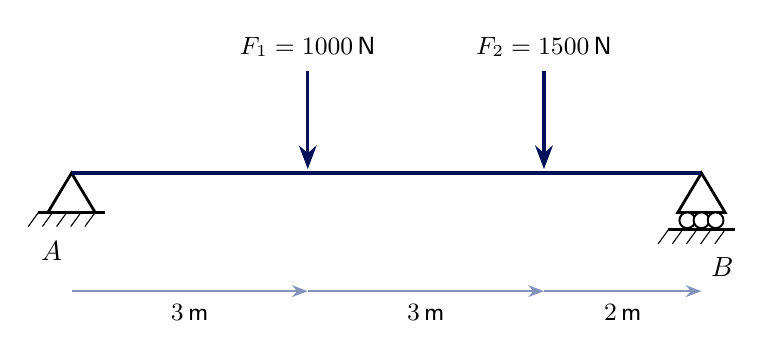
\begin{tikzpicture}
\festlager{(0,0)}
\loslager{(8,0)}
\draw[line width=1.5pt, mainblue] (0,0) -- (8,0);
\node[below left] at (0,-0.75) {$A$};
\node[below right] at (8,-0.95) {$B$};
\draw[force] (3,1.3) -- (3,0.05);
\node[above] at (3,1.35) {\small $F_1=1000\,\text{N}$};
\draw[force] (6,1.3) -- (6,0.05);
\node[above] at (6,1.35) {\small $F_2=1500\,\text{N}$};
\draw[dim] (0,-1.5) -- (3,-1.5);
\node[below] at (1.5,-1.55) {\small $3\,\text{m}$};
\draw[dim] (3,-1.5) -- (6,-1.5);
\node[below] at (4.5,-1.55) {\small $3\,\text{m}$};
\draw[dim] (6,-1.5) -- (8,-1.5);
\node[below] at (7,-1.55) {\small $2\,\text{m}$};
\end{tikzpicture}

% ================= Ex 4.1 FBD (Schnittbild) =================
\begin{tikzpicture}
\fill[mainblue] (0,0) circle (2.2pt);
\fill[mainblue] (8,0) circle (2.2pt);
\draw[line width=1.5pt, mainblue] (0,0) -- (8,0);
\node[below left] at (0,-0.15) {$A$};
\node[below right] at (8,-0.15) {$B$};
\draw[force] (0,-1.1) -- (0,-0.05);
\node[below] at (0,-1.15) {\small $A_y$};
\draw[force] (-1.4,1.2) -- (-0.05,1.2);
\node[left] at (-1.45,1.2) {\small $A_x$};
\draw[force] (8,-1.1) -- (8,-0.05);
\node[below] at (8,-1.15) {\small $B_y$};
\draw[force] (3,1.9) -- (3,0.05);
\node[above] at (3,1.95) {\small $F_1$};
\draw[force] (6,1.9) -- (6,0.05);
\node[above] at (6,1.95) {\small $F_2$};
\end{tikzpicture}

% ================= Ex 4.2 problem: cantilever, fixed support, force + applied moment =================
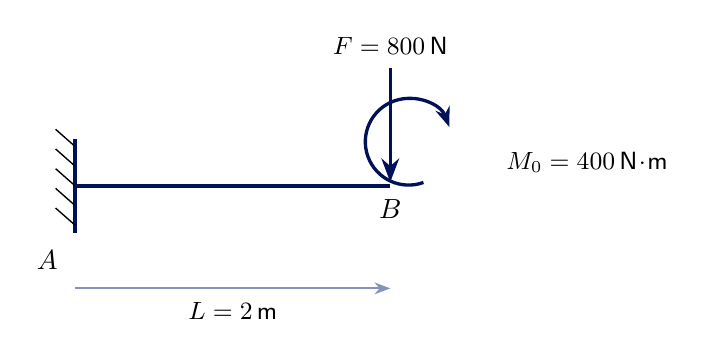
\begin{tikzpicture}
\einspannung{(0,0)}
\draw[line width=1.5pt, mainblue] (0,0) -- (4,0);
\node[below left] at (-0.1,-0.7) {$A$};
\node[below] at (4,-0.05) {$B$};
\draw[force] (4,1.5) -- (4,0.05);
\node[above] at (4,1.55) {\small $F=800\,\text{N}$};
\draw[moment, {Stealth[length=2.5mm]}-] (4.75,0.75) arc (20:290:0.55);
\node[right] at (5.35,0.3) {\small $M_0=400\,\text{N}\!\cdot\!\text{m}$};
\draw[dim] (0,-1.3) -- (4,-1.3);
\node[below] at (2,-1.35) {\small $L=2\,\text{m}$};
\end{tikzpicture}

% ================= Ex 4.2 FBD (Schnittbild) =================
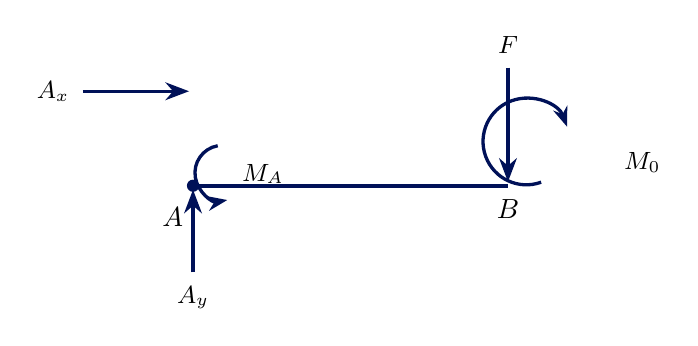
\begin{tikzpicture}
\fill[mainblue] (0,0) circle (2.2pt);
\draw[line width=1.5pt, mainblue] (0,0) -- (4,0);
\node[below left] at (0,-0.15) {$A$};
\node[below] at (4,-0.05) {$B$};
\draw[force] (0,-1.1) -- (0,-0.05);
\node[below] at (0,-1.15) {\small $A_y$};
\draw[force] (-1.4,1.2) -- (-0.05,1.2);
\node[left] at (-1.45,1.2) {\small $A_x$};
\draw[moment, -{Stealth[length=2.5mm]}] (0.314,0.508) arc (100:280:0.35);
\node[right] at (0.5,0.15) {\small $M_A$};
\draw[force] (4,1.5) -- (4,0.05);
\node[above] at (4,1.55) {\small $F$};
\draw[moment, {Stealth[length=2.5mm]}-] (4.75,0.75) arc (20:290:0.55);
\node[right] at (5.35,0.3) {\small $M_0$};
\end{tikzpicture}

% ================= Ex 4.3 problem: beam, pin+roller, full UDL + point load =================
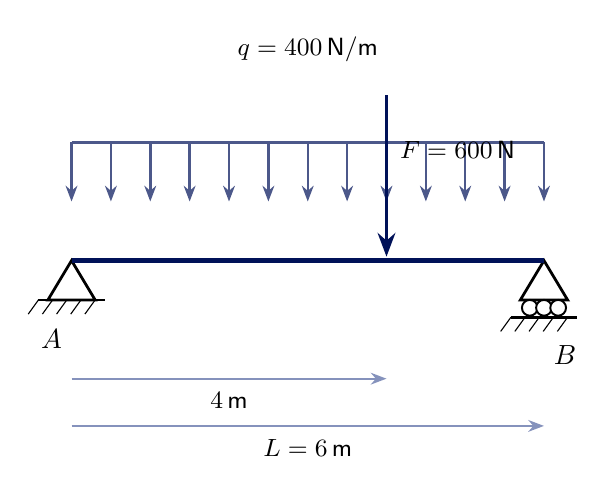
\begin{tikzpicture}
\festlager{(0,0)}
\loslager{(6,0)}
\draw[line width=1.5pt, mainblue] (0,0) -- (6,0);
\node[below left] at (0,-0.75) {$A$};
\node[below right] at (6,-0.95) {$B$};
\qarrows{0}{6}{1.5}{0.75}
\node[above] at (3,2.4) {\small $q=400\,\text{N/m}$};
\draw[force] (4,2.1) -- (4,0.05);
\node[right] at (4.05,1.4) {\small $F=600\,\text{N}$};
\draw[dim] (0,-1.5) -- (4,-1.5);
\node[below] at (2,-1.55) {\small $4\,\text{m}$};
\draw[dim] (0,-2.1) -- (6,-2.1);
\node[below] at (3,-2.15) {\small $L=6\,\text{m}$};
\end{tikzpicture}

% ================= Ex 4.3 FBD (Schnittbild) - q replaced by resultant R =================
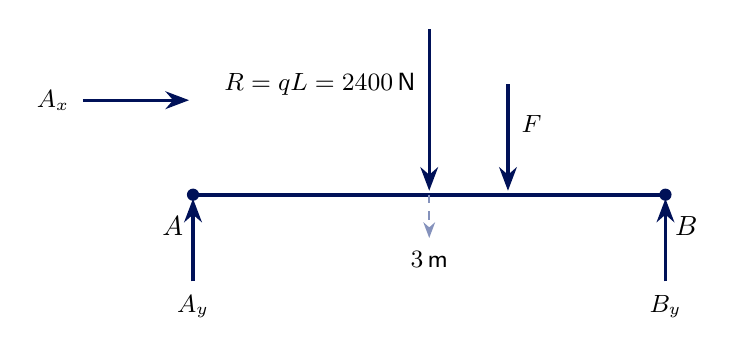
\begin{tikzpicture}
\fill[mainblue] (0,0) circle (2.2pt);
\fill[mainblue] (6,0) circle (2.2pt);
\draw[line width=1.5pt, mainblue] (0,0) -- (6,0);
\node[below left] at (0,-0.15) {$A$};
\node[below right] at (6,-0.15) {$B$};
\draw[force] (0,-1.1) -- (0,-0.05);
\node[below] at (0,-1.15) {\small $A_y$};
\draw[force] (-1.4,1.2) -- (-0.05,1.2);
\node[left] at (-1.45,1.2) {\small $A_x$};
\draw[force] (6,-1.1) -- (6,-0.05);
\node[below] at (6,-1.15) {\small $B_y$};
\draw[force] (3,2.1) -- (3,0.05);
\node[left] at (2.95,1.4) {\small $R=qL=2400\,\text{N}$};
\draw[dim, dashed] (3,0) -- (3,-0.55);
\node[below] at (3,-0.6) {\small $3\,\text{m}$};
\draw[force] (4,1.4) -- (4,0.05);
\node[right] at (4.05,0.9) {\small $F$};
\end{tikzpicture}

% ================= Ex 4.4 problem: beam, pin + link support, partial UDL =================
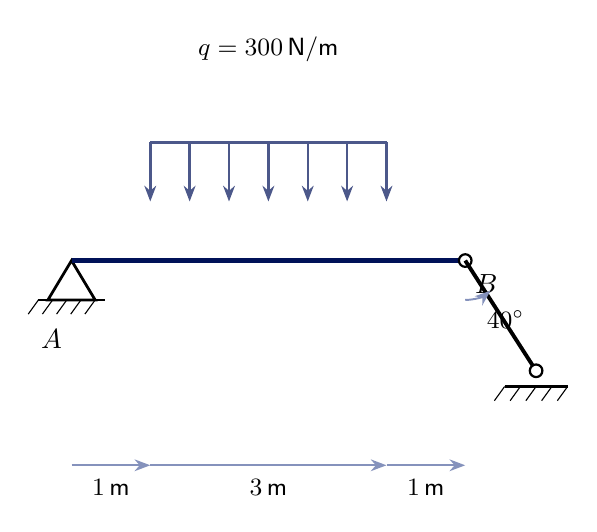
\begin{tikzpicture}
\festlager{(0,0)}
\draw[line width=1.5pt, mainblue] (0,0) -- (5,0);
\node[below left] at (0,-0.75) {$A$};
\node[below right] at (5,-0.05) {$B$};
\draw[fill=white, line width=0.8pt] (5,0) circle (0.08);
\draw[line width=1.4pt] (5,0) -- (5.9,-1.4);
\draw[fill=white, line width=0.8pt] (5.9,-1.4) circle (0.08);
\draw[line width=1pt] (5.5,-1.6) -- (6.3,-1.6);
\foreach \x in {5.5,5.7,...,6.3} {\draw[line width=0.4pt] (\x,-1.6) -- (\x-0.13,-1.78);}
\draw[dim] (5,-0.5) arc (270:310:0.5);
\node[right] at (5.15,-0.75) {\small $40^\circ$};
\qarrows{1}{4}{1.5}{0.75}
\node[above] at (2.5,2.4) {\small $q=300\,\text{N/m}$};
\draw[dim] (0,-2.6) -- (1,-2.6);
\node[below] at (0.5,-2.65) {\small $1\,\text{m}$};
\draw[dim] (1,-2.6) -- (4,-2.6);
\node[below] at (2.5,-2.65) {\small $3\,\text{m}$};
\draw[dim] (4,-2.6) -- (5,-2.6);
\node[below] at (4.5,-2.65) {\small $1\,\text{m}$};
\end{tikzpicture}

% ================= Ex 4.4 FBD (Schnittbild) - q replaced by resultant R, strut force S =================
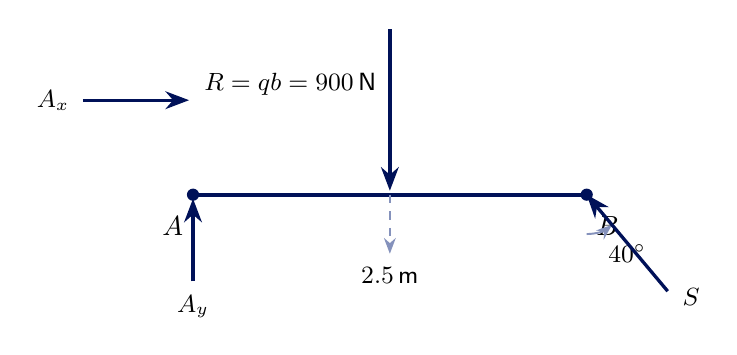
\begin{tikzpicture}
\fill[mainblue] (0,0) circle (2.2pt);
\fill[mainblue] (5,0) circle (2.2pt);
\draw[line width=1.5pt, mainblue] (0,0) -- (5,0);
\node[below left] at (0,-0.15) {$A$};
\node[below right] at (5,-0.15) {$B$};
\draw[force] (0,-1.1) -- (0,-0.05);
\node[below] at (0,-1.15) {\small $A_y$};
\draw[force] (-1.4,1.2) -- (-0.05,1.2);
\node[left] at (-1.45,1.2) {\small $A_x$};
\draw[dim] (5,-0.5) arc (270:310:0.5);
\node[right] at (5.15,-0.75) {\small $40^\circ$};
\draw[force] ($(5,0)+(-50:1.6)$) -- (5,0);
\node[right] at ($(5,0)+(-50:1.7)$) {\small $S$};
\draw[force] (2.5,2.1) -- (2.5,0.05);
\node[left] at (2.45,1.4) {\small $R=qb=900\,\text{N}$};
\draw[dim, dashed] (2.5,0) -- (2.5,-0.75);
\node[below] at (2.5,-0.8) {\small $2.5\,\text{m}$};
\end{tikzpicture}

\end{document}
